\section{Мета практикуму}

Практично ознайомитися із принципами статистичних методiв розрiзнення змiстовного тексту вiд випадкової послiдовностi, порівняти їх.

\subsection{Постановка задачі та варіант}
\begin{tabularx}{\textwidth}{X|X}
	\textbf{Треба виконати} & \textbf{Зроблено} \\
	Знайти достатню кількість текстів українських творів & \checkmark \\
	Реалізувати усі алгоритми розрізнення змістовного тексту & \checkmark \\
	Показати детермінитичну та стохастичну функції & \checkmark \\
	Проаналізувати отримані результати & \checkmark \\
\end{tabularx}



\section{Хід роботи/Опис труднощів}
    У ході роботи над даною лабораторною роботою було:
    \begin{itemize}
        \item зібрано багато текстів українською мовою на 12мб даних;
        \item реалізовано усі критерії за варіантом (1.0-1.3, 3.0, 5.1) + структурний реалізований на алгортимі deflate;
        \item зібрано усі дані та оформлено у один файл.
    \end{itemize}    
    Не можна не сказати про труднощі, що виникали під час виконання роботи, а саме:
    \begin{itemize}
        \item на початку практикуму помилково виконав половину критеріїв із не свого варіанту (4.0, 5.0);  
        \item під час виконання 4.0 критерію так і не зміг знайти у ньому помилку, тому навіть не включав його результати до фінальної таблички;
        \item була спроба зробити ще структурний критерій для алгоритму стиснення lzma, але не вийшло через довгий час роботи;
        \item не можна не згадати про знаходження текстів (витратив багато часу на набір даних для аналізу).
    \end{itemize}


\section{Результати дослідження}
У ході роботи було на практиці реалізовано та використано алгортими для розрізнення змістовного тексту. Проаналізовано та створено узагальнену табличку із результатами.

\section{Особливості реалізації}

Перед тим як говорити про результати роботи критеріїв треба спершу розказати про те як реалізовував їх.
Трохи нижче на картинках можна побачити порогові значення \ref{fig:threshold_values} та таблиці результатів \ref{fig:meanigfull_text}, \ref{fig:vingenere_r1}, \ref{fig:vingenere_r5}, \ref{fig:vingenere_r10}, \ref{fig:affine_substitution}, \ref{fig:random_text}, \ref{fig:recurrent_relation}.
На таблиці результатів та параметрів можна побачити назви критеріїв та їх параметри для виклику. У наступному списку наведу короткий опис як вони були реалізовані та певні нюанси.

\begin{remark}
    У таблиці є наведені певні розбіжності у кількості текстів, що були проаналізовані. Спершу для тих текстів, що бралися із змістовного тексту було проаналізовано увесь текст, уже не став обрізати можливі входи для критеріїв. Саме тому для $L=10$ можна побачити 1 млн входів, але на противагу цьому тексти, що треба було генерувати вручну, то там було виставлено константне значення, що було надане у умові лаборатоної роботи.
\end{remark}

\begin{remark}
    Також у таблиці можна побачити назви, що будуть збивати із пантелику, а саме: $1.3.own$ та $1.1.custom$. Це ідентичні назви, що позначають те, що цей критерій є модифікованим. Причина чому це залишив, не хотів виправляти усі таблички заново. 
\end{remark}

\begin{enumerate}
    \item \textbf{Критерій $1.0$}
        Даний критерій перевіряє певну кількість заборонених $l$-грам на наявність у певному шматку тексту, що містить (10|100|1000|10000) символів. Параметр $h_p$ визначає кількість заборонених біграм, що будуть використані для перевірки тексту на <<справжність>>. У даному випадку для монограм було вибрано всього 8 штук із 32 символів, а для біграм було вибрано 135 шт. із 1024 шт..

        У результаті можна підсумувати, що критерій вів себе так.
        \begin{itemize}
            \item Для змістовного тексту в цілому алгоритм себе показав непогано, але у певних випадках навіть у змістовному тексті познаходило заборонені монограми/біграми. 
            \item Для шифру Віженера із ключем довжини $r=1$ критерій на малих значеннях (для біграм) показав себе погано, так як багато словосполучень було обрізано, а от для великої довжини, що для монограм, що для баграм він справляється досить добре. 
            \item Для шифру Віженера із ключем довжини $r=5$ поведінка у більшості є ідентично до попереднього пункту.
            \item Для шифру Віженера із ключем довжини $r=10$ результат лише змінюється для першого сету $n$-грам. Там лише для біграм у половині випадків можна назвати текст змістовним. 
            \item Для шифру афінної та афінної біграмної підстановки $r=5$ точно так само як попередні критерії для маленьких довжин може давати хибну відповідь.
            \item Для випадкового тексту критерій працює добре, налогічно до попередніх випадків із шифром Віженера.
            \item Для рекурентного співвідношення аналогічна робота відповідно до попереднього критерію.
        \end{itemize}

        У підсумку можна сказати, що цей критерій реалізує примітивну, але досить успішну логіку, що відсікає тексти із $l$-грамами, що зовсім не використовуються у змістовному тексті.

    
    \item \textbf{Критерій $1.0$ модифікований}
        Даний критерій є ідентичним до попереднього, окрім того, що тут змінена перевірка на наявність заборонених монограм/біграм. Дана процедура виконується наступним чином:
        \begin{itemize}
            \item Проходимося по всьому тексту та формуємо геш таблицю із значеннями $l$-грам, що зустрічаються у змістовному тексті. У даному випадку використовував $l = 2, 3, L$;
            \item Далі при перевірці $L$-грами на наявність забороненої $l$-грами перевірялося на нявність заборонених біграм, триграм та $L$-грам, тобто як було знайдено будь-яку заборонену $l$-граму цей текст приймався за випадковий. Сама перевірка на наявність виконуться за допомогою перевірки наявності монограми/біграми, що знаходяться у <<маленькому>> тексті у геш таблиці. Тобто саме ті заборонені $l$-грами, що взагалі не використовуються у змістовному тексті зміожуть відкинути тексти, що були задані певним перетворенням. 
        
        \begin{figure}[!h]
            \centering
            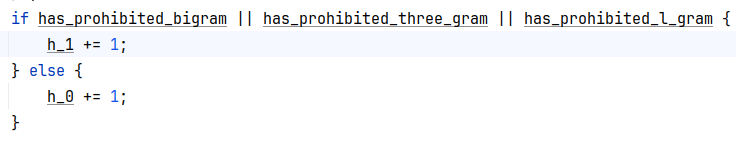
\includegraphics[width=0.5\linewidth]{Images/prh_grams_condition.png}
            \caption{Умова при оновленні значень гіпотез.}
            \label{fig:enter-label}
        \end{figure}
        \end{itemize}

        Параметр $Threshold$ у таблиці параметрів означає мінімальну частоту повторень символу, що повинна бути, для того, щоб вважати знайдені $l$-грами у тексті, за змістовний текст, а не як заборонену $l$-граму. 

        У результаті можна підсумувати, що критерій вів себе так.
        \begin{itemize}
            \item Для змістовного тексту критерій показав себе погано, так як накопичити L-грами досить важко, так як це вимагає великих обчислювальних можливостей. 
            \item Для видозміненого тексту критерій показує себе досить добре, відхиляючи усі можливі тексти. 
        \end{itemize}

        У підсумку можна сказати, що цей критерій погано себе показує на змістовномму тексті, але безпомилково розрізняє видозмінений текст у якому містяться комбінації символів, що взагалі не використовуються у мові.
        
    \item \textbf{Критерій $1.1$}
        Ідея даного критерію полягає у тому, щоб ввести певне порогове значення разом із яким було б простіше визначати змістовні тексти у яких теж може бути певна кількість заборонених біграм. Параметр $k_p$ позначає поріг після якого $L$-грама із кількістю заборонених $l$-грам буде вважатися випадковою, а $h_p$ -- кількість заборонених $l$-грам, що потрібна для перевірки.

         У результаті можна підсумувати, що критерій вів себе наступним чином.
        \begin{itemize}
            \item Для змістовного тексту критерій показав себе добре, адже у більшості текстів не могло набратися значення, що було більше порогового. 
            \item Для видозміненого тексту критерій показує себе досить добре, відхиляючи усі можливі тексти. 
        \end{itemize}

        У підсумку можна сказати, що цей критерій добре себе показує на змістовному та видозмінененому тексті. 
            
    \item \textbf{Критерій $1.1$ модифікований}
        Даний видозмінений алгоритм є подібним до попереднього, лише відрізняється у формі знаходження забороненої $l$-грами у певному тексті. Цей алгоритм подібний до того, що використовується у критерії $1.0.custom$. Тобто текст розподіляється на біграми/триграми/$L$-грами, знаходиться кількість відповідних входжень заборонених граам у певний текст і рахується сума, яка потім перевіряється на умову. Параметр $Threshold$ задає певне порогове значення для таблиці частот, щоб відсіювати дуже малі значення для неї.

        \begin{figure}[!h]
            \centering
            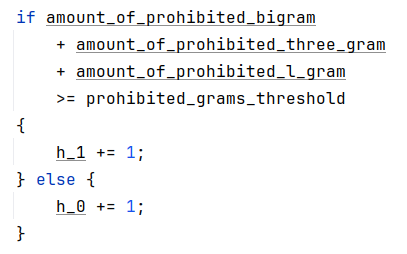
\includegraphics[width=0.5\linewidth]{Images/criterion_1_1_custom.png}
            \caption{Умова для критерію $criterion.1.1.custom$.}
            \label{fig:enter-label}
        \end{figure}

        У результаті можна підсумувати, що критерій вів себе наступним чином.
        \begin{itemize}
            \item Для змістовного тексту критерій показав себе добре, адже у більшості текстів не могло набратися значення, що було більше порогового. 
            \item Для видозміненого тексту критерій показує себе досить погано, лише на  $L=10000$ результат є допустимим. 
        \end{itemize}

        У підсумку можна сказати, що цей критерій добре себе показує на змістовному, але погано на видозміненому тексту із маленькою довжиною. 
        
    \item \textbf{Критерій $1.2$}
        Даний критерій побудований на частотах символів і має свою суть у тому, що якщо у тексті є аномальна кількість заборонених $l$-грам, що буде перевищувати частоту $l$-грами у змістовному тексті, то тоді будемо вважати, що текст є не змістовним. Парметрів даний критерій немає.

        Якщо коротко, то у результаті можна сказати, що критерій лише працює для $l=2$. Це зв'язано із тим фактом, що частоти монограм, або звичайних букв у змістовному тексті є величезними і частоти, що можна здобути у тексті є дуже малими. Вони аж ніяк не можуть преплюнути попередні виміри, напрочут у біграм це виходить. Тому саме цей метод підходить для використання із дво- і більше грамами.
    
    \item \textbf{Критерій $1.2$ модифікований}
        Даний критерій побудований подібним чином до $1.0.custom$ із якого була взята перевірка на наявність забороненої $l$-грами, але основна частина взята із звичайного критерію $1.2$. Параметр $Threshold$ задає певне порогове значення для таблиці частот, щоб відсіювати дуже малі значення для неї. Умова від критерію $1.1.custom$ не змінилася, але змінилося отримання результатів. Саме тут виконується перевірка для біграм/триграм/$L$-грам у паралельних потоках, де шукається невідповідність частот у текстах.

        У результаті можна підсумувати, що критерій вів себе наступним чином.
        \begin{itemize}
            \item Для змістовного тексту критерій показав себе посередньо, адже приблизно половина текстів не приймається за змістовний.
            \item Для видозміненого тексту критерій показує себе добре, адже майже в усіх випадках правильно відрізняє видозмінений текст. 
        \end{itemize}

        У підсумку можна сказати, що цей критерій показує себе посередньо на змістовному тексті, але добре на видозмінених текстах.
        
    \item \textbf{Критерій $1.3$}
        Даний критерій є таким собі узагальненням попередніх і тепер будемо порівнювати аномальну частоту входження $l$-грам у текст в сукупності. Тобто будемо враховувати лише частоти $l$-грам із множини заборонених, яка буде задаватися параметром. Параметромо у даному критерії є $h_H$ -- потужність множини заборонених $l$-грам.

        У результаті можна підсумувати, що критерій вів себе наступним чином.
        \begin{itemize}
            \item Для змістовного тексту критерій показав себе добре, більшість текстів була розпізнана як змістовна.
            \item Для видозміненого тексту критерій показує себе дуже погано, адже у сукупності не може набратися такої кількості частоти, як у звичайному тексті. 
        \end{itemize}

        У підсумку можна сказати, що цей критерій показує себе добре на змістовному тексті, але досить посередньо на видозмінених текстах.
        
    \item \textbf{Критерій $1.3$ модифікований}
        Даний критерій працює так само як і попередній, але як і є у моодифікованих алгоритмів, він використовує інше знаходження заборонених $l$-грам. У моїй реалізації параметр $Threshold$ задає певне порогове значення для таблиці частот, щоб відсіювати дуже малі значення для неї.

        У підсумку можна сказати, що цей критерій показує себе точно так само як не модифікована версія. Тобто добре на довгому змістовному тексті, але досить посередньо на видозмінених текстах.
        
    
    \item \textbf{Критерій $3.0$}
        Саме цей критерій уже увібрав у себе ідею обчислення ентропії на символ джерела $H_i$, що дає обчислювати певну <<узагальнену>> характеристику невизначеності у тексті. Загалом ентропія у змістовному тексті повинна бути майже такою ж самою як у певній частинці. Параметрами у даному критерії виступає певне порогове значення для різниці ентропій, а саме $h_H$.

        У результаті можна підсумувати, що критерій вів себе наступним чином.
        \begin{itemize}
            \item Для змістовного тексту критерій показав себе добре лише для великих текстів, адже на меленьких він не встигає набрати достатні значення для проходження порогу.
            \item Для видозміненого тексту критерій показує себе добре лише для великих текстів, аналогічно як попередній пункт. 
        \end{itemize}

        У підсумку можна сказати, що цей критерій показує себе добре лише на довгих змістовних або видозмінених текстах.
        
    \item \textbf{Критерій $5.0$ та $5.1$}
        Ці два критерії треба розглядати у сукупності так як вони представляють із себе один і той же алгоритм, тільки із різних сторін. Головню суттю цих алгоритмів є виділити певні <<ящики>> і назбирати у них $l$-грами за які буде відповідати ящик. Тобто ящиками у нас будуть виступати певні найменш або найбльш використовувані $l$-грами у змістовному. Також будемо вважати ящик пустим тоді і тільки тоді, коли певні $l$-грама не зустрілася у тексті. Ящики у критерії $5.0$ вибираються як $l$-грами, що зустрічаються найрідше, а у $5.1$ вибираються як щонайчастіше. Щодо параметрів, то у обох алгоритмах використовується параметр $Boxes$, що позначає кількість коробок, які дозволяємо заповнювати та певний поріг $k_{empty}$ -- кількість пустих коробок по якому будемо визначати чи належить текст до випадкового чи ні. 

         У результаті можна підсумувати, що критерій $5.0$ веде себе наступним чином.
        \begin{itemize}
            \item Для змістовного тексту критерій показав себе добре лише для великих текстів, але для біграм якось себе дивно веде (у половині текстів показує, що змістовний текст відображається як випадковий).
            \item Для видозміненого тексту критерій показує себе добре так само лише для текстів із біграмним перетворенням. Із монограмами теж якось не заладилося. 
        \end{itemize}

         А от у критерія $5.1$ спростерігається інша поведінка.
        \begin{itemize}
            \item Для змістовного тексту критерій показав себе посередньо лише для одного із найменших текстів.
            \item Для видозміненого тексту критерій показує себе добре лише для текстів із біграмних перетвореннями на додачу до деяких із монограмних. 
        \end{itemize}
        
        У підсумку можна сказати, що критерій $5.0$ на найрідних $l$-грамах показує себе гірше чим критерій $5.1$ на найчастіших $l$-грамах. Із цього можна вивести висновок, що у випадкових текстах буде якомога менше найбільш частих $l$-грам. 
    
    \item \textbf{Структурний критерій для deflate}
        Почнімо із того, що deflate -- є алгортимом стистення без втрат, що використовує у комбінації алгоритми LZ77 та кодування Гаффмана. Так як це є кодуванням, то воно буде звичайно стискати дані, але на цьому факті можна розрізняти чи був стиснений змістовний текст чи випадковий. Будемо обчислювати коефіцієнт компресії для побудови нашого критерію. Ідея була у тому, що змістовні тексти мають у собі більше різних букв, що дасть змогу лише трохи стиснути текст, а щодо незмістовного можна сказати навпаки. Параметром $Threshold$ тут вистуває певне порогове значення стиснення тексту.

        \begin{figure}[!h]
            \centering
            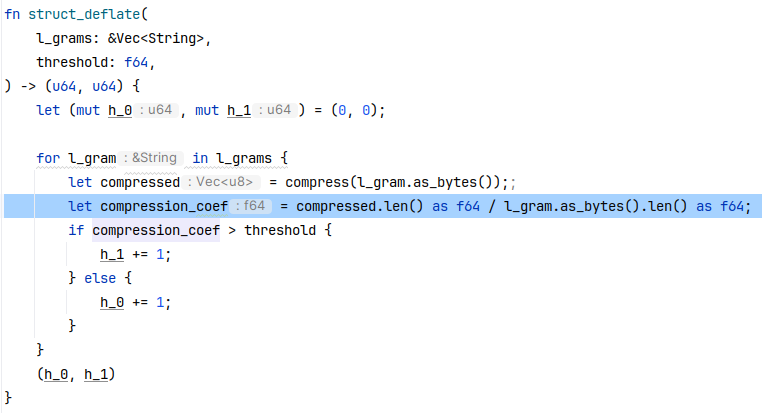
\includegraphics[width=0.5\linewidth]{Images/deflate_algorithm.png}
            \caption{Умова для обчислення структурного критерію.}
            \label{fig:deflate_algorithm}
        \end{figure}

         У результаті можна підсумувати, що цей критерій веде себе наступним чином.
        \begin{itemize}
            \item Для змістовного тексту критерій показав себе загалом добре у всіх випадках.
            \item Для видозміненого тексту критерій показує себе погано для маленьких значень, але для великих досить точно класифікує тексти. 
        \end{itemize}
\end{enumerate}




\subsection{Порогові значення}
\begin{figure}[!h]
    		\centering
    		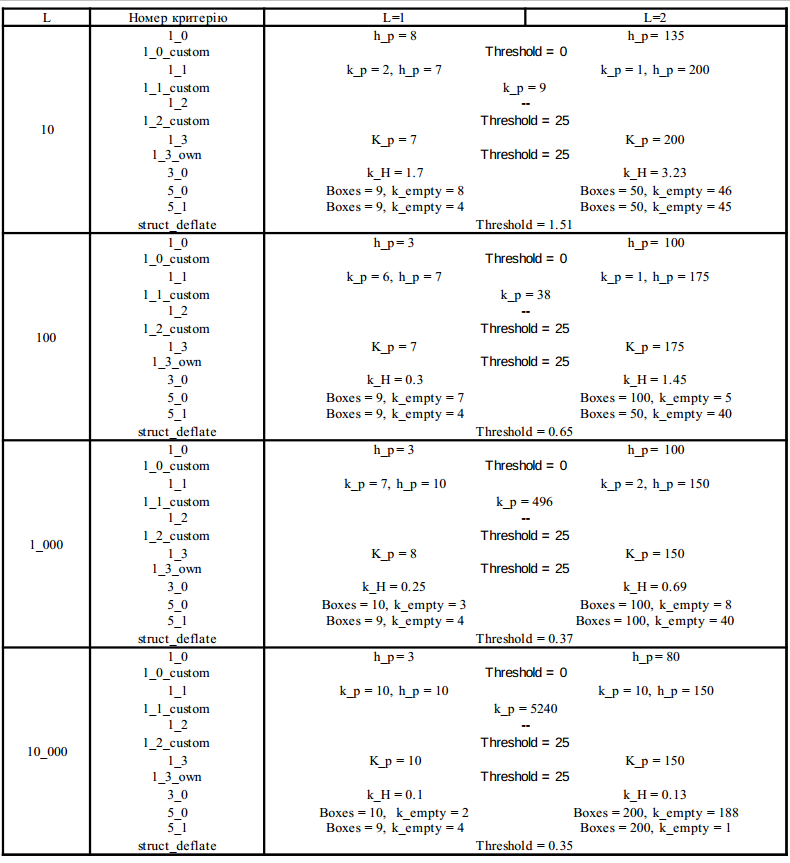
\includegraphics[scale = 0.55]{Images/parameters.png}
    		\caption{Порогові значення для критеріїв.}
    		\label{fig:threshold_values}
	\end{figure}

\subsection{Таблиці із отриманими результатами}

\begin{figure}[!h]
    		\centering
    		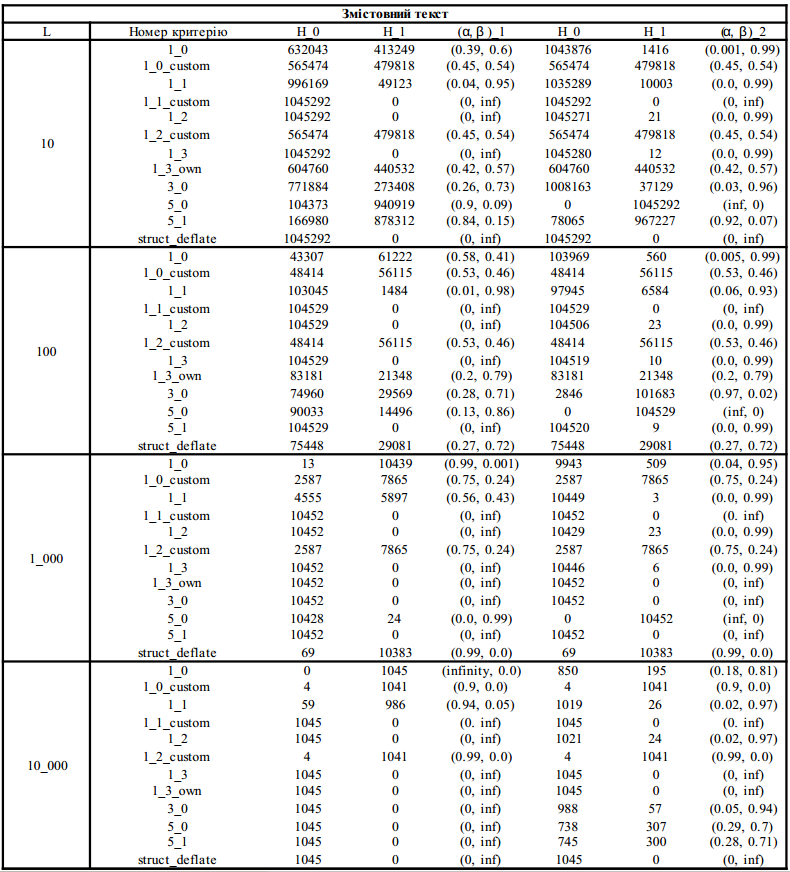
\includegraphics[scale = 0.55]{Images/meaningfull_text.png}
    		\caption{Результати критеріїв для змістовного тексту.}
    		\label{fig:meanigfull_text}
	\end{figure}
 \begin{figure}[!h]
    		\centering
    		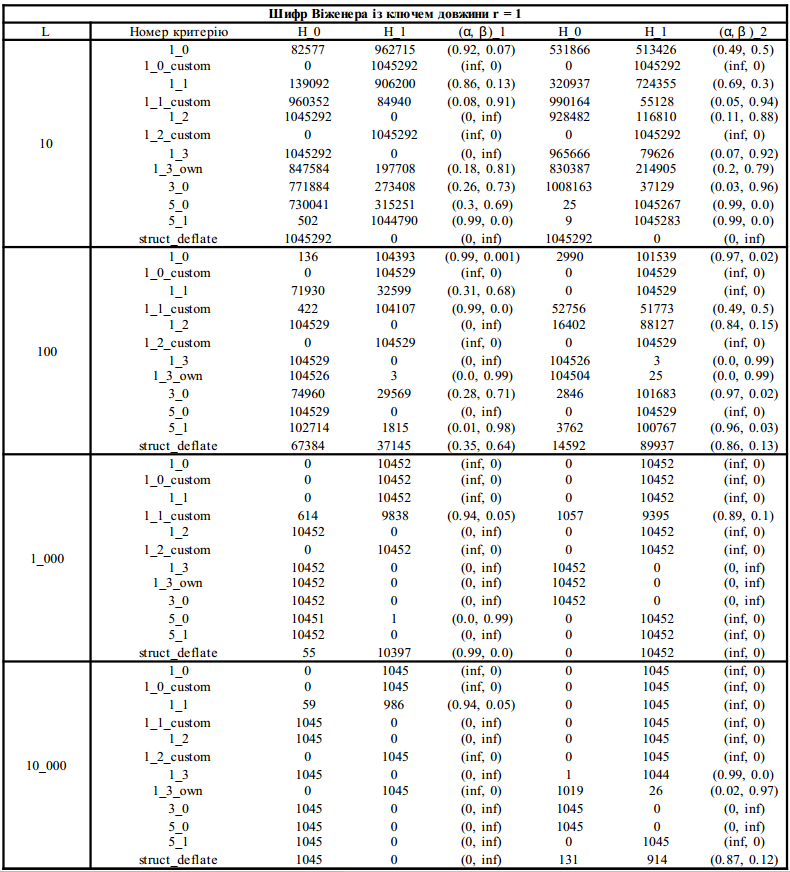
\includegraphics[scale = 0.55]{Images/vingenere_r1.png}
    		\caption{Результати критеріїв для шифру Віженера із ключем довжини $r = 1$.}
    		\label{fig:vingenere_r1}
	\end{figure}
 \begin{figure}[!h]
    		\centering
    		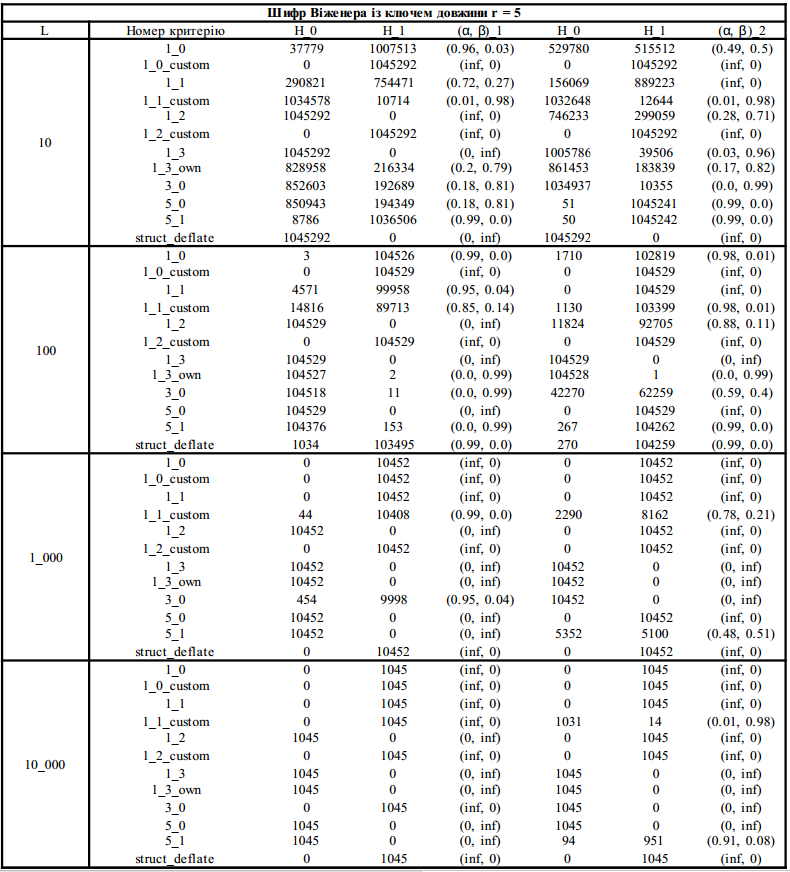
\includegraphics[scale = 0.55]{Images/vingenere_r5.png}
    		\caption{Результати критеріїв для шифру Віженера із ключем довжини $r = 5$.}
    		\label{fig:vingenere_r5}
	\end{figure}
 \begin{figure}[!h]
    		\centering
    		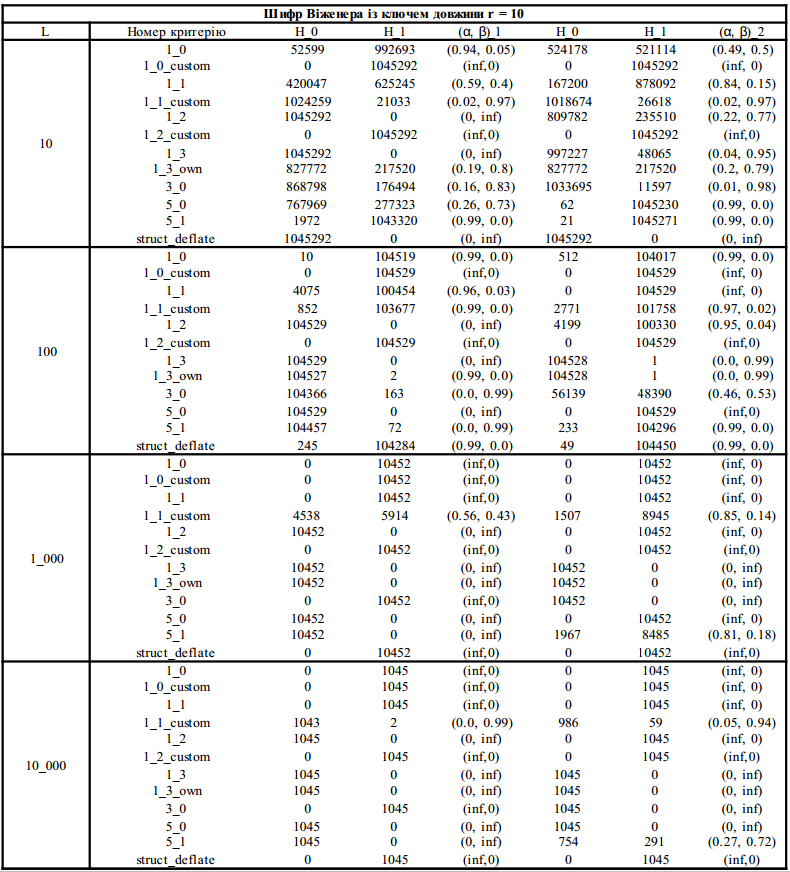
\includegraphics[scale = 0.55]{Images/vingenere_r10.png}
    		\caption{Результати критеріїв для шифру Віженера із ключем довжини $r = 10$.}
    		\label{fig:vingenere_r10}
	\end{figure}
 \begin{figure}[!h]
    		\centering
    		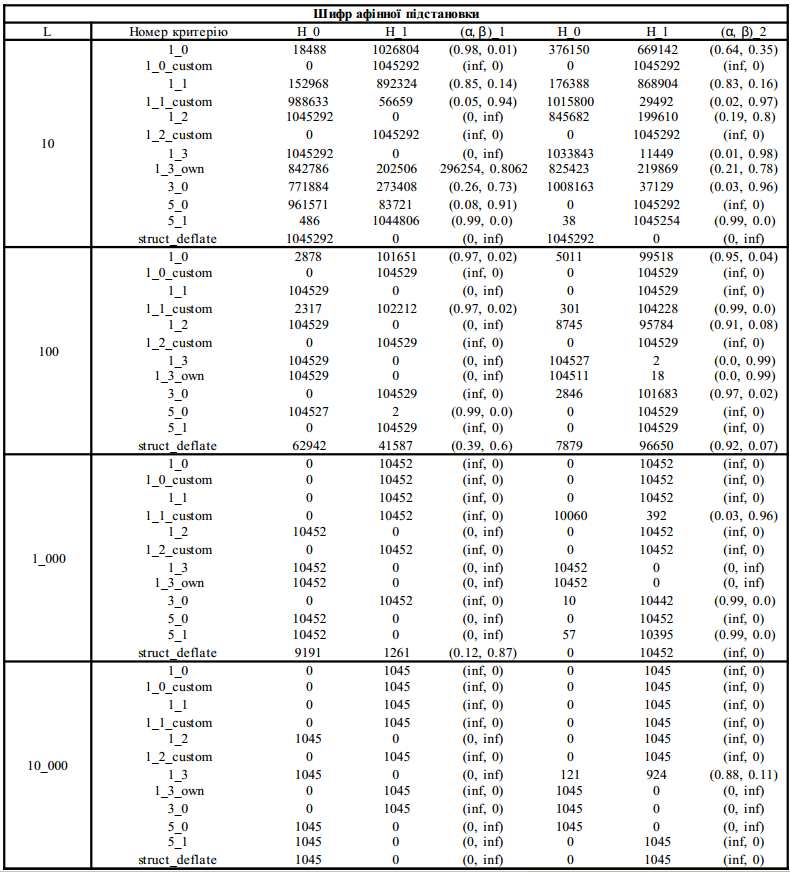
\includegraphics[scale = 0.55]{Images/affine_substitution.png}
    		\caption{Результати критеріїв для шифру афінної та афінної біграмної підстановки.}
    		\label{fig:affine_substitution}
	\end{figure}
 \begin{figure}[!h]
    		\centering
    		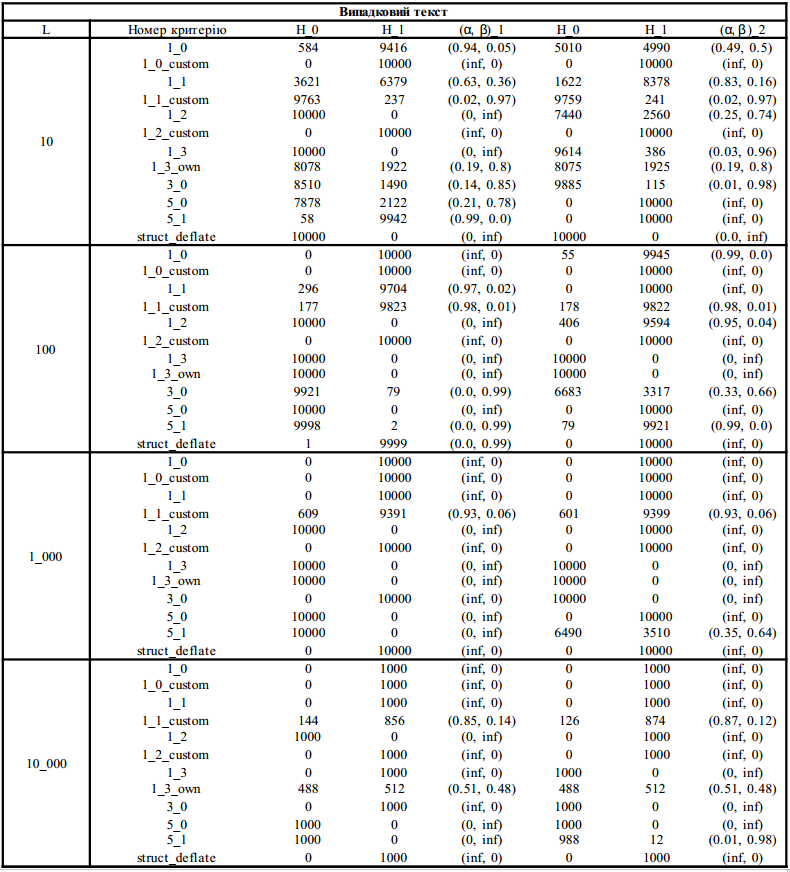
\includegraphics[scale = 0.55]{Images/random_text.png}
    		\caption{Результати критеріїв для випадкового незмістовного тексту тексту.}
    		\label{fig:random_text}
	\end{figure}
 \begin{figure}[!h]
    		\centering
    		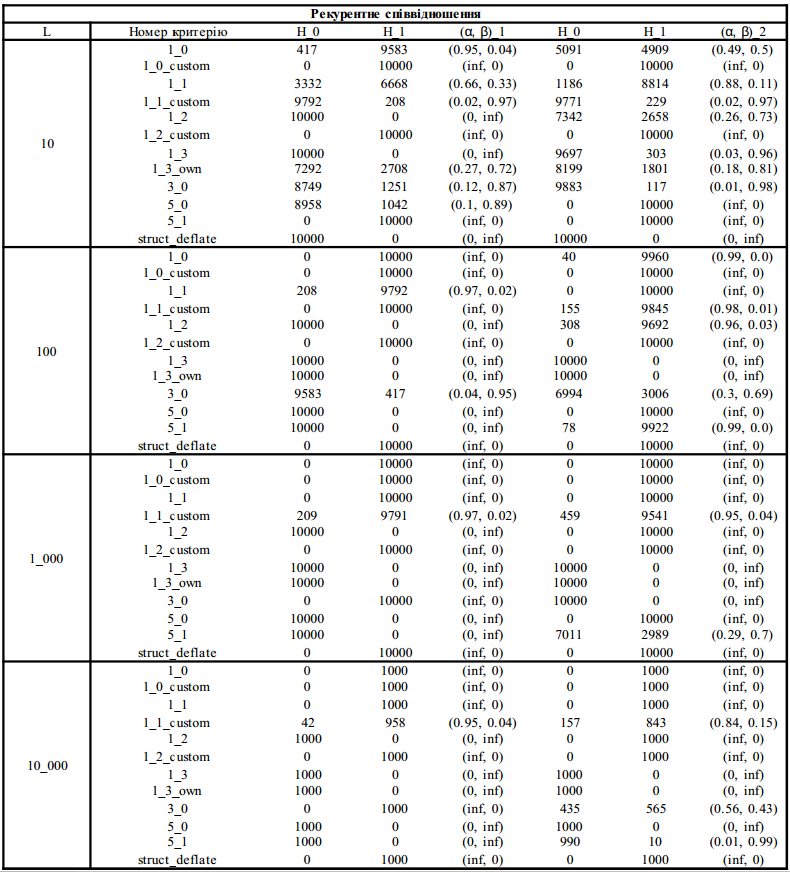
\includegraphics[scale = 0.55]{Images/recurrent_relation.png}
    		\caption{Результати структурних критеріїв для стисненого тексту .}
    		\label{fig:recurrent_relation}
	\end{figure}

\section{Висновки}
За допомогою реалізації практикуму <<Статистичні критерії на відкритий текст>> була можливість побудувати на практиці критерії для перевірки текстів на змістовність тексту та проаналізувати їх роботу у формі аналітичних таблиць. У результаті наведу критерії, які вважаю є сенс використовувати, а які ні для визначення змістовності тексту. 
\begin{itemize}
    \item Рекомендую до використання
        \begin{itemize}
            \item $1.1$ лише на маленьких текстах;
            \item $3.0$ на великих текстах;
            \item $5.1$ на текстах, де є підозра, що перетворення було застосоване біграмне;
            \item $struct.deflate$ на великих текстах.
        \end{itemize} 
    
    \item Не рекомендую до використання або потребує доопрацювання: $1.0$, $1.0.custom$, $1.1.custom$, $1.2$, $1.2.custom$, $1.3$, $1.3.custom$, $5.0$.
\end{itemize}
Щоб покращити загальну роботу критеріїв їх можна використовувати комбіновано, до прикладу, для коротких текстів один критеріїв, для довгих інший або змінювати параметри. 
